\appendix
\renewcommand{\thesection}{\Alph{section}}

\section{Datasets and Evaluation Tables}\label{appendix:datasets}

\subsection{Handcrafted Test Set Sentences}
\label{tab:handcrafted_testset}
\begin{longtable}{|p{6.5cm}|p{6.5cm}|c|}
\hline
\textbf{English} & \textbf{German} & \textbf{Label} \\
\hline
\endfirsthead

\hline
\textbf{English} & \textbf{German} & \textbf{Label} \\
\hline
\endhead

\hline
\multicolumn{3}{|r|}{\textit{Continued on next page}} \\
\hline
\endfoot

\hline
\endlastfoot

\multicolumn{3}{|l|}{\textbf{Neutral}} \\
\hline
Today the weather is beautiful & Heute ist das Wetter schön & 0 \\
I like this guy. & Ich mag diesen Kerl. & 0 \\
How are you? & Wie geht es dir? & 0 \\
BERT is a transformers model pretrained on a large corpus of multilingual data in a self-supervised fashion. & BERT ist ein Transformer-Modell, das auf selbstüberwachte Weise auf einem großen Korpus mehrsprachiger Daten vorab trainiert wird. & 0 \\
Knowledge is love and light and vision. & Wissen ist Liebe und Licht und Vision. & 0 \\
\hline
\multicolumn{3}{|l|}{\textbf{Neutral with Gendered Subjects}} \\
\hline
My mother is an engineer. & Meine Mutter ist Ingenieurin. & 0 \\
Is this boy a good artist? & Ist dieser Junge ein guter Künstler? & 0 \\
I am living with my sister, who is also my best friend & Ich lebe mit meiner Schwester, die auch meine beste Freundin ist & 0 \\
My father was an excellent cook. & Mein Vater war ein ausgezeichneter Koch. & 0 \\
The girls went hiking. & Die Mädchen gingen wandern. & 0 \\
\hline
\multicolumn{3}{|l|}{\textbf{Biased}} \\
\hline
Do you like our maths teacher? & Mögen Sie unsere Mathelehrerin? & 1 \\
The doctor was late to work today. & Der Arzt kam heute zu spät zur Arbeit. & 1 \\
Tomorrow the students are leaving for a class trip. & Morgen gehen die Studenten zu einer Klassenfahrt. & 1 \\
This nurse does not work hard. & Diese Krankenschwester arbeitet nicht hart. & 1 \\
Athletes earn a lot of money. & Sportler verdienen viel Geld. & 1 \\
\hline
\multicolumn{3}{|l|}{\textbf{GFL Variants}} \\
\hline
Engineers are kind and hard-working & Ingenieur*innen sind lieb und fleißig & 0 \\
Engineers are kind and hard-working & Ingenieure und Ingenieurinnen sind lieb und fleißig & 0 \\
Teachers are kind and hard-working & Lehrende sind lieb und fleißig & 0 \\
Teachers are kind and hard-working & Lehrer:innen sind lieb und fleißig & 0 \\
Teachers are kind and hard-working & Lehrerinnen und Lehrer sind lieb und fleißig & 0 \\
Teachers are kind and hard-working & Lehrer sind lieb und fleißig & 1 \\
Teachers are kind and hard-working & Lehrerinnen sind lieb und fleißig & 1 \\
\hline
\multicolumn{3}{|l|}{\textbf{Job Posting (Real-world)}} \\
\hline
We’re seeking someone to join our team Office 365 squads to lead the design, development, and integration of Gen AI apps and integration using Microsoft Copilot Studio. & Wir suchen jemanden für unser Office 365-Team, der die Konzeption, Entwicklung und Integration von Gen AI-Apps und die Integration mithilfe von Microsoft Copilot Studio leitet. & 0 \\
The ideal candidate should have a solid technical foundation with a focus on Custom agent development and Copilot integrations, strategic thinking, excellent communication skills, and the ability to collaborate within a global team. & Der ideale Kandidat sollte über solide technische Grundlagen mit Schwerpunkt auf der Entwicklung kundenspezifischer Agenten und Copilot-Integrationen, strategisches Denken, ausgezeichnete Kommunikationsfähigkeiten und die Fähigkeit zur Zusammenarbeit in einem globalen Team verfügen. & 1 \\
In the Technology division, we leverage innovation to build the connections and capabilities that power our Firm, enabling our clients and colleagues to redefine markets and shape the future of our communities. & Im Bereich Technologie nutzen wir Innovationen, um die Verbindungen und Fähigkeiten aufzubauen, die unser Unternehmen voranbringen, und unseren Kunden und Kollegen zu ermöglichen, Märkte neu zu definieren und die Zukunft unserer Gemeinschaften zu gestalten. & 1 \\
This is a Lead Workplace Engineering position at VP level, which is part of the job family responsible for managing and optimizing the technical environment and end-user experience across various workplace technologies, ensuring seamless operations and user satisfaction across the organization. & Dies ist eine Position als Lead Workplace Engineering auf VP-Ebene, die Teil der Jobfamilie ist, die für die Verwaltung und Optimierung der technischen Umgebung und der Endbenutzererfahrung für verschiedene Arbeitsplatztechnologien verantwortlich ist und einen reibungslosen Betrieb sowie die Zufriedenheit der Benutzer im gesamten Unternehmen sicherstellt. & 1 \\
\end{longtable}


\subsection{Performance of Dataset Tuning Test Runs}
\label{appendix:dataset_tuning_table}
\begin{table}[h]
\centering
\begin{tabularx}{\textwidth}{lXXXXX}
\hline
Metric & Dataset A & Dataset B & Dataset C & Dataset D & Dataset E \\
\hline
Macro F1 & 0.972 & 0.966 & 0.953 & 0.956 & 0.969 \\
Accuracy (held-out) & 0.972 & 0.967 & 0.955 & 0.957 & 0.976 \\
Accuracy (handcrafted) & 0.808 & 0.808 & 0.769 & 0.808 & 0.808 \\
\hline
\end{tabularx}
\caption{Evaluation results for datasets A-E.}
\end{table}

\subsection{False Positives and False Negatives from Held-out Test Set}
\label{tab:fp_fn_table}
\begin{longtable}{|l|p{6cm}|p{6cm}|}
\hline
Error Type & English Text & German Text \\
\hline
\endfirsthead
\hline
Error Type & English Text & German Text \\
\hline
\endhead
False Positive & Accordingly, the President of the French Republic, the President of the European Council and the French Prime Minister asked me to visit, before the President of the French Republic, the ten countries which are currently asking for only one commissioner. & In diesem Sinne haben das Oberhaupt der Republik, die Präsidentschaft des Europäischen Rates und das französische Regierungsoberhaupt mich beauftragt, vor der Rundreise des Oberhaupts der Republik die zehn Länder aufzusuchen, die gegenwärtig nur einen Kommissionssitz beanspruchen. \\
False Positive & In so doing, we are beginning to train the next generation of police officers to work and operate throughout Europe; in other words, we will be preparing them to implement Community law and joint and Community actions. & Wir beginnen also jetzt mit der Ausbildung der nächsten Generation von Polizeibeamteten, die in der Lage sein sollen, auf europäischer Ebene zu arbeiten und zu handeln, d. h. sie werden darauf vorbereitet, das Gemeinschaftsrecht anzuwenden und die gemeinsamen und gemeinschaftlichen Maßnahmen umzusetzen. \\
False Positive & The Heads of State and Government therefore agreed a number of measures to promote the development of risk capital in the European Union, with a deadline for implementing the Risk Capital Action Plan of 2003. & Die Staats - und Regierungoberhäupter beschlossen deshalb eine Reihe von Maßnahmen zur Förderung der Entwicklung von Risikokapital in der Europäischen Union, um den Risikokapital - Aktionsplan bis zum Jahr 2003 vollständig umzusetzen. \\
False Positive & We will, over the coming weeks, have to take account of the results of the dialogue between the two political leaders, or of the absence of such a dialogue. & In den kommenden Wochen werden wir die Ergebnisse des Dialogs zwischen den beiden politischen Spitzen bzw. das Ausbleiben eines solchen Dialogs zur Kenntnis nehmen müssen. \\
False Positive & Would you go for treatment to somebody who knows all the surgical terms in Italian, English, French and German, or would you go to a surgeon? & Würden Sie sich von einem Menschen, der sich ausgezeichnet in den chirurgischen Fachbegriffen in Italienisch, Französisch und Deutsch auskennt, oder von einem Menschen, der als Chirurg ausgebildet wurde, operieren lassen? \\
False Positive & I have just been to the station to see my uncle off. & Ich war gerade am Bahnhof, um mich von meinem Onkel zu verabschieden. \\
False Positive & The specialists are intelligent. & Die Sachkundigen sind intelligent. \\
False Positive & The recipient is responsible. & Rezipierende ist verantwortlich. \\
False Positive & What we still need are more experts to guide our companies through complex procedures at European level. & Was wir noch brauchen, sind weitere Fachleute, die unseren Betrieben in schwierigen Prozessen auf europäischer Ebene helfen. \\
False Positive & I shall try very briefly to pinpoint a few political aspects of the four areas touched on in greater or lesser detail by all the speakers, i.e. the new political approach in the social agenda, secondly the content, thirdly the means and fourthly the procedures. & Ich werde versuchen, in aller Kürze einige politische Bemerkungen zu den vier Themenbereichen vorzutragen, die mehr oder weniger ausführlich von allen, die das Wort hatten, angesprochen wurden. Es sind dies erstens das neue politische Konzept der sozialpolitischen Agenda, zweitens der Inhalt, drittens die Mittel und viertens die Verfahren. \\
False Negative & Here too the local people are frustrated by the immigration of Muslims and the hard line taken by the military. & Hier wird die lokale Bevölkerung ebenfalls durch die Zuwanderung von Muslimen und das unnachsichtige Auftreten des Militärs schwer gebeutelt. \\
\hline
\caption{All false positives and false negatives from the test set}
\end{longtable}


\subsection{Handcrafted Test Set Results}
\label{tab:handcrafted_testset_results}
\begin{table}[H]
\centering
\label{tab:hc_test_results}
\begin{tabular}{clllccr}
\toprule
\# & English (short) & True & Predicted & Neutral & Biased & Correct \\
\midrule
0  & Today weather is beautiful             & 0 & 0 & 0.9996 & 0.0004 & yes \\
1  & I like this guy                        & 0 & 0 & 0.9997 & 0.0003 & yes \\
2  & How are you?                          & 0 & 0 & 0.9998 & 0.0002 & yes \\
3  & BERT transformers model               & 0 & 0 & 0.6888 & 0.3112 & yes \\
4  & Knowledge is love and light           & 0 & 0 & 0.9992 & 0.0008 & yes \\
5  & My mother is an engineer              & 0 & 1 & 0.4412 & 0.5588 & no  \\
6  & Is this boy a good artist?            & 0 & 0 & 0.6223 & 0.3777 & yes \\
7  & I live with my sister                  & 0 & 0 & 0.9988 & 0.0012 & yes \\
8  & My father was an excellent cook       & 0 & 0 & 0.9080 & 0.0920 & yes \\
9  & The girls went hiking                  & 0 & 0 & 0.9986 & 0.0014 & yes \\
10 & Do you like our maths teacher?        & 1 & 1 & 0.0917 & 0.9083 & yes \\
11 & The doctor was late today              & 1 & 1 & 0.0007 & 0.9993 & yes \\
12 & Tomorrow students leaving              & 1 & 1 & 0.0007 & 0.9993 & yes \\
13 & This nurse does not work hard          & 1 & 1 & 0.0017 & 0.9983 & yes \\
14 & Athletes earn a lot of money           & 1 & 1 & 0.0012 & 0.9988 & yes \\
15 & Engineers are kind (GFL form)          & 0 & 0 & 0.9541 & 0.0459 & yes \\
16 & Engineers are kind (neutral plural)    & 0 & 1 & 0.0008 & 0.9992 & no  \\
17 & Teachers are kind (neutral)             & 0 & 0 & 0.9973 & 0.0027 & yes \\
18 & Teachers are kind (colon form)          & 0 & 1 & 0.0314 & 0.9686 & no  \\
19 & Teachers are kind (explicit plural)     & 0 & 1 & 0.0005 & 0.9995 & no  \\
20 & Teachers are kind (male plural)          & 1 & 1 & 0.0008 & 0.9992 & yes \\
21 & Teachers are kind (female plural)        & 1 & 1 & 0.0007 & 0.9993 & yes \\
22 & Seeking someone for Office 365 team      & 0 & 0 & 0.9964 & 0.0036 & yes \\
23 & Ideal candidate with solid foundation    & 1 & 1 & 0.0006 & 0.9994 & yes \\
24 & Technology division leverages innovation & 1 & 1 & 0.0004 & 0.9996 & yes \\
25 & Lead Workplace Engineering position      & 1 & 1 & 0.0015 & 0.9985 & yes \\
\bottomrule
\end{tabular}
\caption[Handcrafted test set results]{Handcrafted test set results: model predictions and confidence scores}
\end{table}



% -------------
\section{Use of Artificial Intelligence}\label{appendix:artificial_intelligece}

\subsection{Perplexity.ai for Literature Research}
Prompting perplexity.ai for further sources on Gender Bias in English to German Machine Translation and LLMs. 

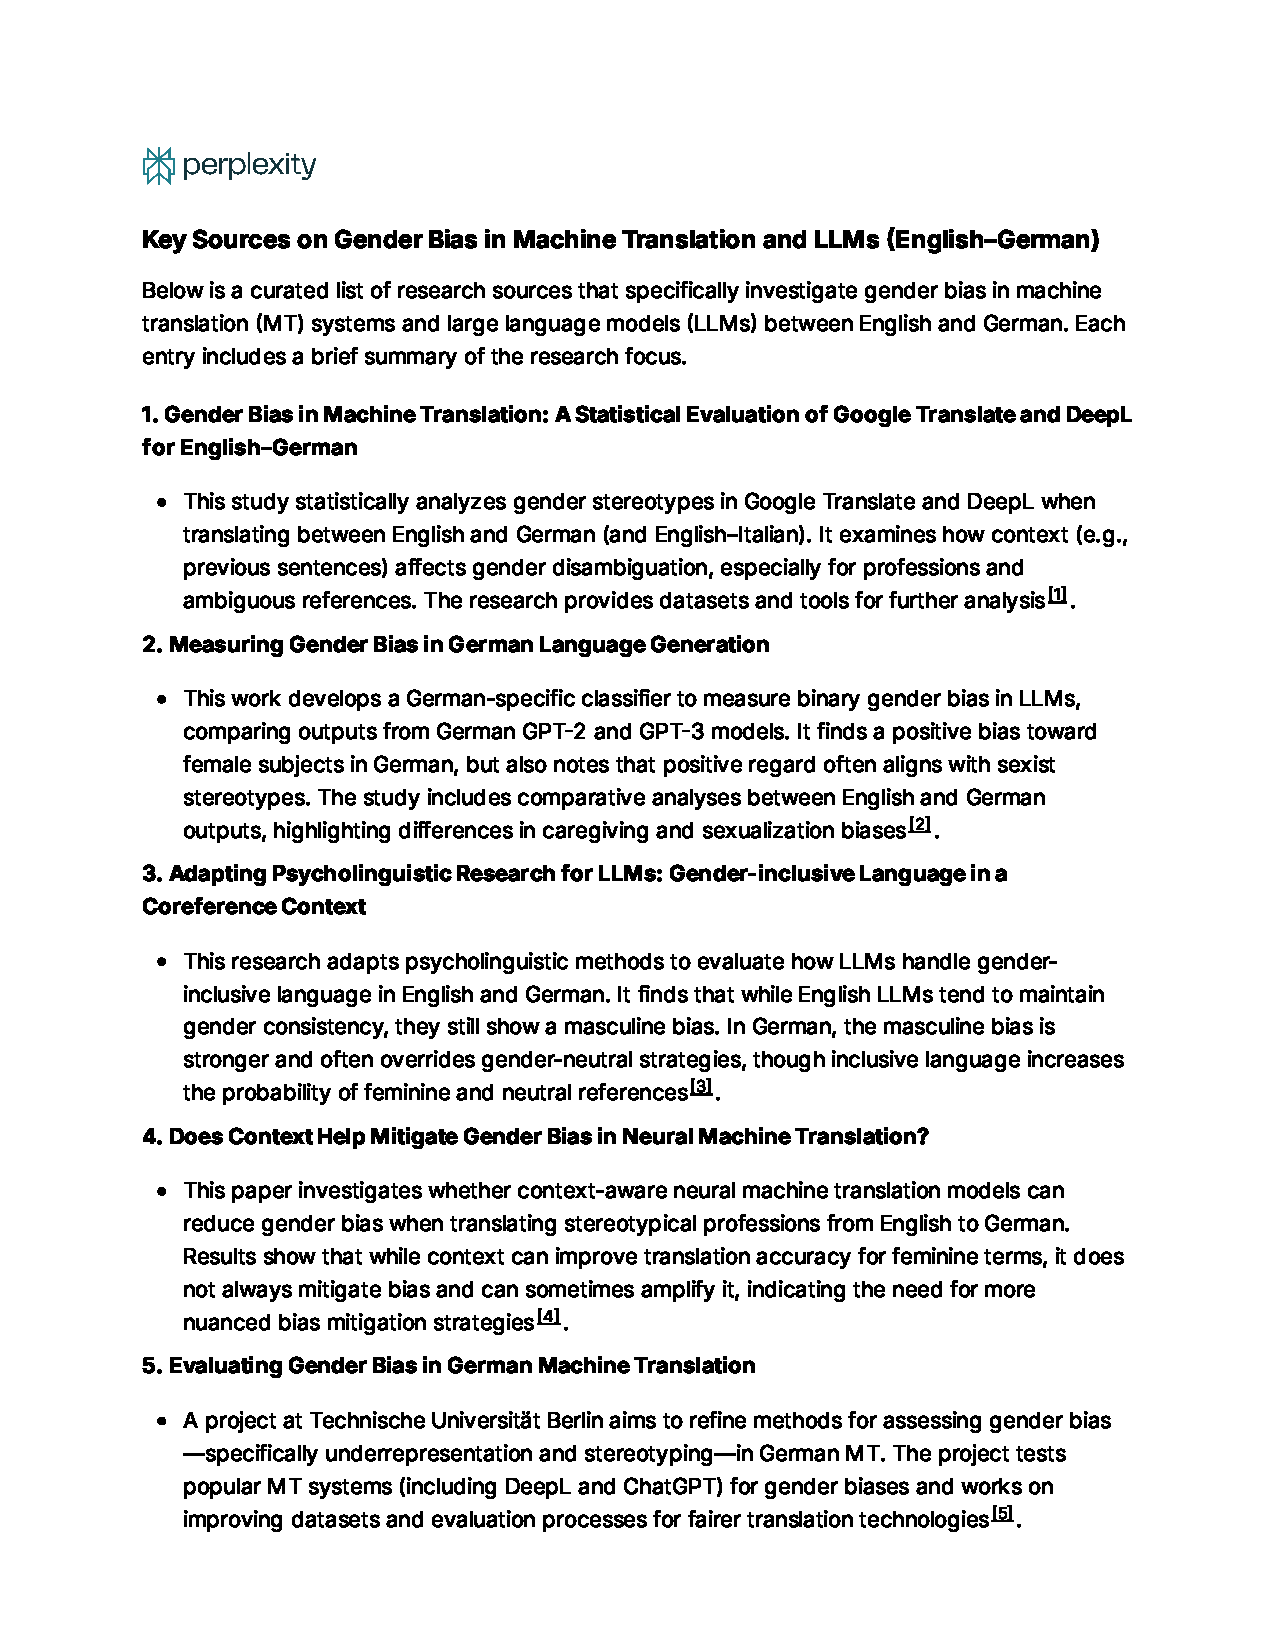
\includepdf[pages=-]{./Literatur/Key Sources on Gender Bias in Machine Translation 21-may-2025.pdf}

\subsection{Use of AI for Code Generation}\label{appendix:ai_code}
During the development of the practical part, ChatGPT and DeepSeek were used to assist in generating portions of the implementation surrounding the demo, specifically in \texttt{app.py}, \texttt{utils.py}, and \texttt{translate.py}. The process was iterative, involving multiple rounds of suggestions and refinements. All AI-generated code was reviewed, adapted, and integrated by the author to ensure correctness and suitability for the project. AI assistance was limited to supporting implementation and did not replace the author’s own programming work or design decisions. In the following, one example of AI-assisted code generation is provided. Due to the iterative nature of the process, not all intermediate outputs can be shown. This example is intended to give a general sense of how AI was used to support the implementation.

\subsubsection{Prompt: } 

\begin{lstlisting}
look at my app.py: 
import streamlit as st
import torch
from transformers import BertTokenizer, BertForSequenceClassification
from utils import split_sentences, predict_bias_batch

device = torch.device("cuda" if torch.cuda.is_available() else "cpu")
MODEL_DIR = "./model_output" 
MAX_LENGTH = 128
BIAS_CONF_THRESHOLD = 0.9

@st.cache_resource(show_spinner=False)
def load_model_and_tokenizer():
    tokenizer = BertTokenizer.from_pretrained(MODEL_DIR)
    model = BertForSequenceClassification.from_pretrained(MODEL_DIR)
    model.to(device)
    model.eval()
    return tokenizer, model

tokenizer, model = load_model_and_tokenizer()

st.title("English to German Translation with Gender Bias Detection")
text = st.text_area("Enter English text here:")

if st.button("Translate"):
    if not text.strip():
        st.write("Please enter some text")
    else:
        st.write("### Results")
        sentences = split_sentences(text)
        results = predict_bias_batch(tokenizer, model, sentences, max_length=MAX_LENGTH, device=device, bias_threshold=BIAS_CONF_THRESHOLD)

        for sentence, translation, pred, conf in results:
            st.write(f"**english:** {sentence}")
            st.write(f"**german:** {translation}")
            if pred == 1 and conf >= BIAS_CONF_THRESHOLD:
                st.warning(f"Bias detected confidence: {conf:.2f}")
            else:
                st.success(f"No bias detected confidence: {conf:.2f}")
            st.markdown("---")

and utils.py:

import re
from translate import translate
import torch

def split_sentences(text):
    # split on . ! or ? followed by space(s)
    sentences = re.split(r'(?<=[.!?])\s+', text.strip())
    return [s for s in sentences if s]

def predict_bias_batch(tokenizer, model, sentences, max_length=128, device='cpu', bias_threshold=0.9):
    results = []
    for sentence in sentences:
        translation = translate(sentence)
        inputs = tokenizer(
            sentence,
            translation,
            return_tensors="pt",
            truncation=True,
            padding="max_length",
            max_length=max_length,
        )
        inputs = {k: v.to(device) for k, v in inputs.items()}
        with torch.no_grad():
            outputs = model(**inputs)
            probs = torch.softmax(outputs.logits, dim=1)
            pred = torch.argmax(probs, dim=1).item()
            confidence = probs[0][pred].item()
        results.append((sentence, translation, pred, confidence))
    return results

right now there is only one input field that utilises the translate script. i want another option that the user can choose to manually input translation, for example a tab selection. there are two input fields where the user inputs english and german and click a button "check bias". then the same standard bias detection script runs. you may add a new file or change existing ones
\end{lstlisting}

\subsubsection{Output:}
\begin{lstlisting}
To add the option for manual translation input, use Streamlit's `st.tabs` to create two modes:

1. **Translate Mode** (uses your `translate()` function).
2. **Manual Input Mode** (user provides both English and German text).

You only need to slightly update `app.py` and optionally refactor `predict_bias_batch` to handle one or more pairs directly. You do **not** need to change `utils.py` unless you want cleaner logic separation.

import streamlit as st
import torch
from transformers import BertTokenizer, BertForSequenceClassification
from utils import split_sentences, predict_bias_batch

device = torch.device("cuda" if torch.cuda.is_available() else "cpu")
MODEL_DIR = "./model_output"
MAX_LENGTH = 128
BIAS_CONF_THRESHOLD = 0.9

@st.cache_resource(show_spinner=False)
def load_model_and_tokenizer():
    tokenizer = BertTokenizer.from_pretrained(MODEL_DIR)
    model = BertForSequenceClassification.from_pretrained(MODEL_DIR)
    model.to(device)
    model.eval()
    return tokenizer, model

tokenizer, model = load_model_and_tokenizer()

st.title("Gender Bias Detection in English-German Translations")

tab1, tab2 = st.tabs(["Translate", "Manual Input"])

with tab1:
    text = st.text_area("Enter English text here:")
    if st.button("Translate and Check Bias"):
        if not text.strip():
            st.write("Please enter some text")
        else:
            st.write("### Results")
            sentences = split_sentences(text)
            results = predict_bias_batch(
                tokenizer,
                model,
                sentences,
                max_length=MAX_LENGTH,
                device=device,
                bias_threshold=BIAS_CONF_THRESHOLD,
                use_translation=True,
            )
            for sentence, translation, pred, conf in results:
                st.write(f"**english:** {sentence}")
                st.write(f"**german:** {translation}")
                if pred == 1 and conf >= BIAS_CONF_THRESHOLD:
                    st.warning(f"Bias detected confidence: {conf:.2f}")
                else:
                    st.success(f"No bias detected confidence: {conf:.2f}")
                st.markdown("---")

with tab2:
    manual_en = st.text_area("Enter English sentence:")
    manual_de = st.text_area("Enter German translation:")
    if st.button("Check Bias"):
        if not manual_en.strip() or not manual_de.strip():
            st.write("Please enter both English and German text")
        else:
            result = predict_bias_batch(
                tokenizer,
                model,
                [(manual_en, manual_de)],
                max_length=MAX_LENGTH,
                device=device,
                bias_threshold=BIAS_CONF_THRESHOLD,
                use_translation=False,
            )[0]
            sentence, translation, pred, conf = result
            st.write(f"**english:** {sentence}")
            st.write(f"**german:** {translation}")
            if pred == 1 and conf >= BIAS_CONF_THRESHOLD:
                st.warning(f"Bias detected confidence: {conf:.2f}")
            else:
                st.success(f"No bias detected confidence: {conf:.2f}")
\end{lstlisting}
